
%%~~~~~~~~~~~~~~~~~~~~~~~~~~~~~~~~~~~~
%\begin{document}
\chapter{Tips and Tricks for analyses in R related to the {\tt MRSea} Package}
\label{cha:tips}


%~~~~~~~~~~~~~~~~~~~~~~~~~~~~~~~~~~~~~~~~~
%~~~~~~~~~~~~~~~~~~~~~~~~~~~~~~~~~~~~~~~~~~~
\section{Distance Tips and Tricks}
\subsection{Analysing binned distance data}
\noindent If we decide to bin the exact distance data into intervals and fit a detection function to interval distance data we can do this by first adding the cut points of the respective interval for each detection to the data using the function {\tt which.bin} and then setting the argument {\tt binned} within {\tt meta.data} to {\tt TRUE}. Note that for the new version of {\tt mrds}, the cut points of the intervals also need to be defined with the argument {\tt breaks} when running the function. 
\begin{knitrout}\footnotesize
\definecolor{shadecolor}{rgb}{0.969, 0.969, 0.969}\color{fgcolor}\begin{kframe}
\begin{alltt}
\hlfunctioncall{data}(dis.data.re)
dis.data.re<-\hlfunctioncall{which.bin}(dis.data.re, cutpoints=c(0,50,100,150,200,250))
result.int<-\hlfunctioncall{ddf}(dsmodel=~mcds(key="hn",formula=~1),data=dis.data.re, 
    method="ds", meta.data=list(width=250, binned=T, 
     breaks=c(0,50,100,150,200,250)))
\end{alltt}
\end{kframe}
\end{knitrout}

\noindent The AIC value from this model may not be compared with the AIC from a model which uses exact distance data from the offshore worked example due to the fact that the data have changed by binning the distances.  \\

\subsection{Plotting side by side detection function plots for different factor covariate levels}
\noindent We begin with the example from the worked example above where we fit a covariate model to the exact distance data. We use the following {\tt ddf} call which includes the two level factor covariate {\tt impact} in the detection function model. We then plot the two detection functions for the respective levels side by side: 
\begin{knitrout}\footnotesize
\definecolor{shadecolor}{rgb}{0.969, 0.969, 0.969}\color{fgcolor}\begin{kframe}
\begin{alltt}
\hlfunctioncall{data}(dis.data.re)
result.imp<-\hlfunctioncall{ddf}(dsmodel=~mcds(key="hn", formula=~1+impact), 
     data=dis.data, method="ds", meta.data=list(width=250))
par(mfrow=c(1,2))
plot(result.imp, showpoints=F, breaks=seq(0,250,25), subset=impact==0, 
    main="Before Impact")
plot(result.imp, showpoints=F, breaks=seq(0,250,25), subset=impact==1, 
    main="After Impact")
\end{alltt}
\end{kframe}
\end{knitrout}
\begin{figure}[h]
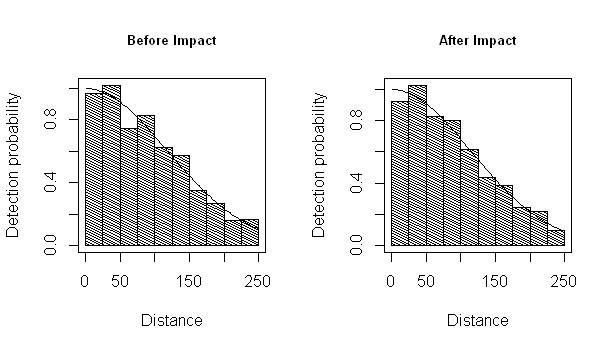
\includegraphics[width=12cm]{impactdetplot.png}
\end{figure}
%~~~~~~~~~~~~~~~~~~~~~~~~~~~~~~~~~~~~~~~~~
%~~~~~~~~~~~~~~~~~~~~~~~~~~~~~~~~~~~~~~~~~~~

\section{Spatial Modelling Tips and Tricks}
\subsection{General}

\begin{block}{Use of {\tt grep} function}
the {\tt grep} function is used in the following {\tt MRSea} functions: {\tt getPvalues}, {\tt plotCumRes}, {\tt plotRunsProfile}, {\tt runPartialPlots} and {\tt runSALSA1D} .  This will cause the user some issues if there are nested covariate names in the model. \\

For example:  
\begin{itemize}
\item wavefront and wavefrontheight are not suitable as wavefront is nested,
\item but wavefront and waveheight are fine.
\end{itemize}
\end{block}

% ~~~~~~~~~~~~~~~~~~~~~~~~~~~~~~~~~
\begin{block}{Save option for plotting}
\noindent All of the plotting functions in {\tt MRSea} have an option for saving a 'png' image straight to your working directory. See the help files of specific functions for details.

\noindent For example:
\begin{knitrout}\footnotesize
\definecolor{shadecolor}{rgb}{0.969, 0.969, 0.969}\color{fgcolor}\begin{kframe}
\begin{alltt}
\hlfunctioncall{plotCumRes}(fullModel, varlist, splineParams, save=T, label=\hlstring{'_glmk1'})
\end{alltt}
\end{kframe}
\end{knitrout}
\end{block}

\noindent This code will save cumulative residual plots for residuals ordered by all variables specified in {\tt varlist} and by predicted value and temporal order into the working directory.  The label allows the user to make the file name specific to the model.  In this case, one of the plots is labelled `CumRes\_observationhour\_glmk1.png'.


\subsection{SALSA}
\label{tips:subsec:salsa}
\begin{block}{SALSA1D knots}
When smoothing biological data many people will restrict the degrees of freedom to reflect the unlikely nature of more complex smooths.  For this reason, and our experience gained from using SALSA on biological data, we recommend that the maximum number of knots for a one-dimensional smooth is between 3 and 5.
\end{block}

\begin{block}{SALSA2D knots}
Requirements for the SALSA2D knot grid:
\begin{itemize}
\item {\tt (k x 2)} data frame
\item regular grid covering whole study region
\begin{itemize}
\item {\tt c(NA, NA)} in rows where the knot location is invalid
\item Invalid is on land 
\item or very far away from data
\end{itemize}
\end{itemize}
\end{block}

\noindent Make a grid that covers the study region
\begin{knitrout}\footnotesize
\definecolor{shadecolor}{rgb}{0.969, 0.969, 0.969}\color{fgcolor}\begin{kframe}
\begin{alltt}
\hlcomment{# load data}
\hlfunctioncall{data}(dis.data.re)
\hlfunctioncall{data}(predict.data.re)

\hlcomment{# sequence of x and y values spaced by 2000 (roughly the spacing of the 
     transects)}
x<-\hlfunctioncall{seq}(\hlfunctioncall{min}(dis.data.re$x.pos), \hlfunctioncall{max}(dis.data.re$x.pos), by=2000)
y<-\hlfunctioncall{seq}(\hlfunctioncall{min}(dis.data.re$y.pos), \hlfunctioncall{max}(dis.data.re$y.pos), by=2000)
grid<-\hlfunctioncall{expand.grid}(x.pos=x, y.pos=y)

\hlfunctioncall{plot}(dis.data.re$x.pos, dis.data.re$y.pos, pch=20, cex=0.5, asp=1, 
     xlab=\hlstring{x.pos'}, ylab=\hlstring{'y.pos'})
\hlfunctioncall{points}(grid, pch=20, col=\hlstring{'red'})

\hlcomment{# draw round boundary as no boundary polygon available}
bnd<-\hlfunctioncall{locator}() 
\hlcomment{# i have drawn the coastline to the top for the boundary}
\hlfunctioncall{polymap}(bnd, add=T)
\end{alltt}
\end{kframe}
\end{knitrout}

\noindent First find the knot points that are on land (Figure \ref{fig:knot1}).

\begin{knitrout}\footnotesize
\definecolor{shadecolor}{rgb}{0.969, 0.969, 0.969}\color{fgcolor}\begin{kframe}
\begin{alltt}
marker<-\hlfunctioncall{rep}(0, \hlfunctioncall{nrow}(grid))
id<-\hlfunctioncall{which}(\hlfunctioncall{inout}(grid, bnd)==TRUE)
\hlcomment{# place a 1 in the marker vector for knots we do not want}
marker[id]<-1

\hlcomment{# make knotgrid object and make unwanted knot locations NA}
knotgrid<-grid
knotgrid[marker==1,]<-\hlfunctioncall{c}(NA,NA)
\end{alltt}
\end{kframe}
\end{knitrout}

\begin{figure}
\centering
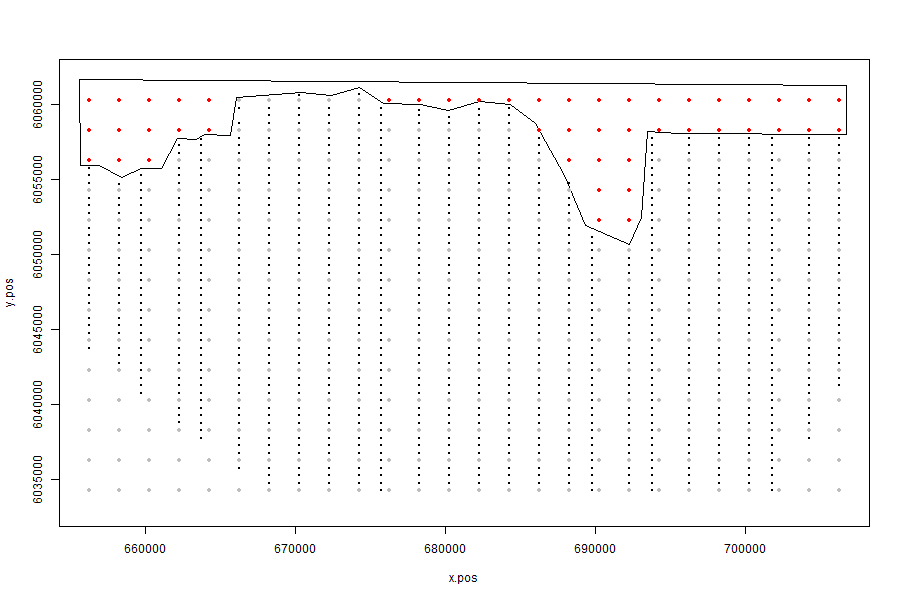
\includegraphics[width=9cm]{knot1.png}
\caption{Figure identifying knot locations inside a boundary (red).  The grey dots are knot locations outside the boundary and the black dots are the data locations.}
\label{fig:knot1}
\end{figure}

\noindent There are still knots in the open water area to the bottom of the survey.  The Euclidean distance between knots and data is used to identify knots that are located a specified distance from any data.  These knot locations are identified as illegal by placing an NA row in the knot grid object. The final knot grid is given in Figure \ref{fig:knot2}. 
\begin{knitrout}\footnotesize
\definecolor{shadecolor}{rgb}{0.969, 0.969, 0.969}\color{fgcolor}\begin{kframe}
\begin{alltt}
distcheck<-\hlfunctioncall{makeDists}(datacoords=\hlfunctioncall{cbind}(dis.data.re$x.pos, dis.data.re$y.pos), 
     knotcoords=\hlfunctioncall{na.omit}(knotgrid))

naid<-\hlfunctioncall{which}(\hlfunctioncall{is.na}(knotgrid[,1]))
\hlcomment{# knots further tham 1km from data are identified with a 1}
marker[-naid][\hlfunctioncall{which}(\hlfunctioncall{apply}(distcheck$dataDist, 2, \hlfunctioncall{min})>1000)]<-1
knotgrid[marker==1,]<-\hlfunctioncall{c}(NA,NA)
\end{alltt}
\end{kframe}
\end{knitrout}

\begin{figure}
\centering
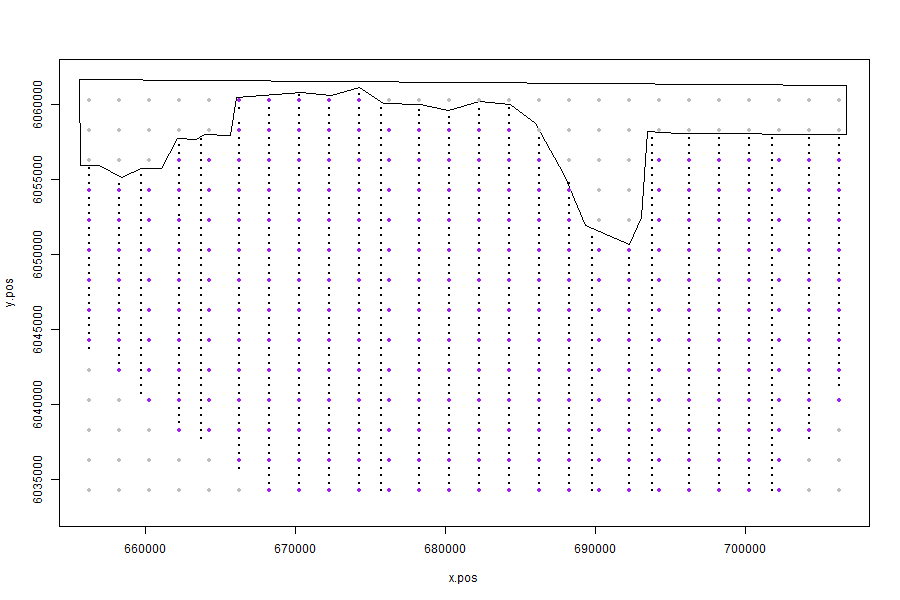
\includegraphics[width=9cm]{knot3.png}
\caption{Figure identifying legal (purple) and illegal (grey) knot locations.  The black dots are the data locations.}
\label{fig:knot2}
\end{figure}

% ~~~~~~~~~~~~~~~~~~~~~~~~~~~~~~~~~
\begin{block}{{\tt gap} parameter}
The gap parameter was discussed briefly in section \ref{subsec:offmodseln} (page \pageref{gappage}) to prevent adjacent knots when there was no data between transects.  Whilst the example was for SALSA2D, {\tt gap} is also an argument for SALSA1D.  Occasionally, knots may be placed too close causing prediction error.  The user may specify a gap in the {\tt salsa1dlist} or {\tt salsa2dlist} arguments to prevent this.  The specification of a gap may also reduce computational time, since there are fewer legal moves for a knot.
\end{block}

%~~~~~~~~~~~~~~~~~~~~~~~~~~~~~
\begin{block}{Interaction Terms}
More than one interaction term may be included, however the code for SALSA2D may only be run on one interaction at a time.  Furthermore, the knot locations selected for the spatial smooth in one interaction term will also be used for any other interaction terms.
\end{block}
% ~~~~~~~~~~~~~~~~~~~~~~~~~~~~~~~~~
\subsection{SALSA1D with more than one smooth covariate}

The examples presented in chapters \ref{cha:off} and \ref{cha:near} fitted only one smooth covariate.  The following code describes how two or more smooth covariates may be added to the model using {\tt runSALSA1D} to select the smoothness (knot locations) for each.\\

\noindent There are two ways to run models with more than one smooth covariate:

\begin{enumerate}
\item No removal of terms from the model.  Useful if SALSA1D is only required for knot selection and the user decides on variable selection.
\item Variable selection included.  The resulting model may have terms removed, be linear or smooth.
\end{enumerate}

\noindent Both methods are set up in the same way:

\noindent Start by building the spline parameters object and specifying more than one covariate in {\tt varlist}.
\begin{knitrout}\footnotesize
\definecolor{shadecolor}{rgb}{0.969, 0.969, 0.969}\color{fgcolor}\begin{kframe}
\begin{alltt}
\hlcomment{# make splineParams object}
splineParams<-\hlfunctioncall{makesplineParams}(data=data, varlist=\hlfunctioncall{c}(\hlstring{'observationhour'},
    \hlstring{'DayOfMonth'}), predictionData=predictData)
\hlfunctioncall{str}(splineParams)
\begin{verbatim}
List of 3
 $ : list()
 $ :List of 5
  ..$ covar      : chr "observationhour"
  ..$ explanatory: int [1:27798] 12 8 9 10 11 12 13 14 15 8 ...
  ..$ knots      : num 12
  ..$ bd         : int [1:2] 4 20
  ..$ degree     : num 2
 $ :List of 5
  ..$ covar      : chr "DayOfMonth"
  ..$ explanatory: int [1:27798] 13 16 16 16 16 16 19 19 19 25 ...
  ..$ knots      : num 13.9
  ..$ bd         : int [1:2] 1 31
  ..$ degree     : num 2
\end{verbatim}
\end{alltt}
\end{kframe}
\end{knitrout}

\noindent To fit a simple model with the default knot values (one knot at the mean) simply repeat the {\tt bs()} term, used in the previous examples, one for each covariate.

\begin{knitrout}\footnotesize
\definecolor{shadecolor}{rgb}{0.969, 0.969, 0.969}\color{fgcolor}\begin{kframe}
\begin{alltt}
\hlcomment{# fitting a model with two smooth terms}
fullModel<-\hlfunctioncall{glm}(birds ~ \hlfunctioncall{as.factor}(floodebb) + \hlfunctioncall{as.factor}(impact) + 
    \hlfunctioncall{bs}(observationhour, knots=splineParams[[2]]$knots) + 
    \hlfunctioncall{bs}(DayOfMonth, knots=splineParams[[3]]$knots) + 
    x.pos + y.pos, family=quasipoisson, data=data)
\end{alltt}
\end{kframe}
\end{knitrout}

\noindent To run SALSA with more than one covariate there are changes in the {\tt salsa1dlist} object and in the {\tt varlist} argument of {\tt runSALSA1D}.  Each covariate must be specified in {\tt varlist} and {\tt minKnots\_1d}, {\tt maxKnots\_1d}, {\tt startKnots\_1d}, {\tt degree} and {\tt gaps} must all be vectors the same length as {\tt varlist}.  This allows different parameters for each of the covariates.\\

\noindent Below is an example of the two ways to run SALSA when you have more than one smooth covariate:

\begin{block}{1. No removal of terms}
\noindent Each covariate is added to the model as a smooth term with the knots specified in the spline parameter object (default knot at the mean if from {\tt makesplineParams}) and then SALSA checks each one in turn for an improvement in knot number and location.  If there is an improvement then the spline parameter object is updated with the new number and location.\\

\noindent Note: There must be a {\tt foldid} column in the data so that cross-validation can be used for selection.

\begin{knitrout}\footnotesize
\definecolor{shadecolor}{rgb}{0.969, 0.969, 0.969}\color{fgcolor}\begin{kframe}
\begin{alltt}
data$response<- data$birds
\hlcomment{# set initial model without the spline terms in there}
initialModel <- \hlfunctioncall{glm}(response ~ \hlfunctioncall{as.factor}(floodebb) + \hlfunctioncall{as.factor}(impact) + 
    \hlfunctioncall{offset}(\hlfunctioncall{log}(area)), family = \hlstring{"quasipoisson"}, data = data)

salsa1dlist<-\hlfunctioncall{list}(fitnessMeasure = \hlstring{"QICb"}, minKnots_1d=\hlfunctioncall{c}(2,2), 
                  maxKnots_1d = \hlfunctioncall{c}(20, 20), startKnots_1d = \hlfunctioncall{c}(2,2), 
                  degree=\hlfunctioncall{c}(2,2), maxIterations = 10, gaps=\hlfunctioncall{c}(1,1))

\hlcomment{# run SALSA}
salsa1dOutput <- \hlfunctioncall{runSALSA1D}(initialModel, salsa1dlist, varlist=
    \hlfunctioncall{c}(\hlstring{"observationhour"}, \hlstring{"DayOfMonth"}), factorlist=\hlfunctioncall{c}(\hlstring{"floodebb"}, \hlstring{"impact"}), 
    predictData,  splineParams=splineParams)
\end{alltt}
\end{kframe}
\end{knitrout}

\noindent The structure of the output is the same as before but with more information in {\tt modelFits1D} regarding what terms were fitted and what knots were chosen.

\begin{knitrout}\footnotesize
\definecolor{shadecolor}{rgb}{0.969, 0.969, 0.969}\color{fgcolor}\begin{kframe}
\begin{alltt}
\hlfunctioncall{str}(salsa1dOutput, max.level = 1)
\begin{verbatim}
List of 4
 $ bestModel   :List of 30
  ..- attr(*, "class")= chr [1:2] "glm" "lm"
 $ modelFits1D :List of 3
 $ splineParams:List of 3
 $ fitStat     : num 31627
\end{verbatim}
\end{alltt}
\end{kframe}
\end{knitrout}

\noindent We can also look directly at the SALSA selected knots by looking at the spline parameter object.  In this example, three knots were chosen for observation hour, whilst the knot location for day of the month was unchanged from the default value (the mean).  One must now consider whether or not day of the month should be a model covariate at all by fitting a model with and without it or using the {\tt runSALSA1D\_withremoval} code instead (below).

\begin{knitrout}\footnotesize
\definecolor{shadecolor}{rgb}{0.969, 0.969, 0.969}\color{fgcolor}\begin{kframe}
\begin{alltt}
\hlcomment{# knots chosen for observation hour}
salsa1dOutput$splineParams[[2]]$knots
\begin{verbatim}
[1]  9 15 17
\end{verbatim}
\hlcomment{# knots chosen for day of month}
salsa1dOutput$splineParams[[3]]$knots
\begin{verbatim}
[1]  13.86
\end{verbatim}
\end{alltt}
\end{kframe}
\end{knitrout}
\end{block}

\begin{block}{2. Removal of terms}
\noindent Each covariate is added to the model as a smooth term with the knots specified in the spline parameter object (default knot at the mean if from {\tt makesplineParams}) and then SALSA checks each one in turn for an improvement in knot number and location.  If there is an improvement then the spline parameter object is updated with the new number and location. If there is no improvement over the single mean knot model then the term is tested as linear or with the term removed.  The model with the best CV score is returned as {\tt salsa1dOutput\$bestModel} (in the example below).

\begin{knitrout}\footnotesize
\definecolor{shadecolor}{rgb}{0.969, 0.969, 0.969}\color{fgcolor}\begin{kframe}
\begin{alltt}
data$response<- data$birds
data$blockid<-pastedata$transect.id, data$season, data$impact, sep="")
data$foldid<-getCVids(data, folds=5, block='blockid')
\hlcomment{# set initial model without the spline terms in there}
initialModel <- \hlfunctioncall{glm}(response ~ \hlfunctioncall{as.factor}(floodebb) + \hlfunctioncall{as.factor}(impact) + 
    \hlfunctioncall{offset}(\hlfunctioncall{log}(area)), family = \hlstring{"quasipoisson"}, data = data)

salsa1dlist<-\hlfunctioncall{list}(fitnessMeasure = \hlstring{"QICb"}, minKnots_1d=\hlfunctioncall{c}(2,2), 
                  maxKnots_1d = \hlfunctioncall{c}(20, 20), startKnots_1d = \hlfunctioncall{c}(2,2), 
                  degree=\hlfunctioncall{c}(2,2), maxIterations = 10, gaps=\hlfunctioncall{c}(1,1))

\hlcomment{# run SALSA}
salsa1dOutput <- \hlfunctioncall{runSALSA1D_withremoval}(initialModel, salsa1dlist, varlist=
    \hlfunctioncall{c}(\hlstring{"observationhour"}, \hlstring{"DayOfMonth"}), factorlist=\hlfunctioncall{c}(\hlstring{"floodebb"}, \hlstring{"impact"}), 
    predictData,  splineParams=splineParams)
\end{alltt}
\end{kframe}
\end{knitrout}

\noindent The structure of the output is the same as before but with more information in {\tt modelFits1D} regarding what terms were kept and if knots were chosen and an additional entry, {\tt keptvarlist}, listing the covariates retained in the best model.

\begin{knitrout}\footnotesize
\definecolor{shadecolor}{rgb}{0.969, 0.969, 0.969}\color{fgcolor}\begin{kframe}
\begin{alltt}
\hlfunctioncall{str}(salsa1dOutput, max.level = 1)
\begin{verbatim}
List of 5
 $ bestModel   :List of 30
  ..- attr(*, "class")= chr [1:2] "glm" "lm"
 $ modelFits1D :List of 3
 $ splineParams:List of 3
 $ fitStat     : num 31951
 $ keptvarlist : chr "observationhour"
\end{verbatim}
\end{alltt}
\end{kframe}
\end{knitrout}

\noindent The model selected has removed DayOfMonth and selects 3 knots for observationhour. To see what happened during the process look at the {\tt modelFits1D} object in the output.  The first step (list entry 1) fitted a model with the knot values in {\tt splineParams}.  In this case that is one knot at the mean for each covariate.

\footnotesize
\begin{verbatim}
> salsa1dOutput$modelFits1D
[[1]]
[[1]]$term
[1] "startmodel"

[[1]]$kept
NULL

[[1]]$basemodelformula
glm(formula = response ~ as.factor(floodebb) + as.factor(impact) + 
   offset(log(area)) + bs(observationhour, knots = splineParams[[2]]$knots, 
   degree = splineParams[[2]]$degree, Boundary.knots = splineParams[[2]]$bd) 
   + bs(DayOfMonth, knots = splineParams[[3]]$knots, degree = 
   splineParams[[3]]$degree, Boundary.knots = splineParams[[3]]$bd), 
   family = quasipoisson,  data = data)

[[1]]$knotsSelected
NULL

[[1]]$tempfits
         CV     fitStat 
   33.89111 32564.32819 
\end{verbatim}
\normalsize

\noindent The second step (list entry 2) investigates new knot locations and numbers for observationhour.  Three knots were selected by SALSA and kept in the model due to an improvement in CV score from the step above (33.89 to 33.83).  The {\tt baseModelFits} (model returned from this step) and {\tt modelfits} (model with knots chosen by SALSA) are identical as the new knots are retained.

\footnotesize
\begin{verbatim}
[[2]]
[[2]]$term
[1] "bs(observationhour, knots = splineParams[[2]]$knots, 
      degree=splineParams[[2]]$degree, Boundary.knots=splineParams[[2]]$bd)"

[[2]]$kept
[1] "YES - new knots"

[[2]]$basemodelformula
glm(formula = response ~ as.factor(floodebb) + as.factor(impact) + 
    bs(DayOfMonth, knots = splineParams[[3]]$knots, degree = 
    splineParams[[3]]$degree, Boundary.knots = splineParams[[3]]$bd) 
   + bs(observationhour, knots = splineParams[[2]]$knots, degree = 
    splineParams[[2]]$degree, Boundary.knots = splineParams[[2]]$bd) 
   + offset(log(area)), family = quasipoisson, data = data)

[[2]]$knotsSelected
[1]  9 15 16

[[2]]$baseModelFits
         CV     fitStat 
   33.83714 31627.38018 

[[2]]$modelfits
         CV     fitStat 
   33.83714 31627.38018 
\end{verbatim}
\normalsize

\noindent The last step (list entry 3 in this example)  investigates new knot locations and numbers for DayOfMonth.  A smooth term is not retained as the CV score is worse for the selected knots (33.84) and improves over the model from the previous step when the term is removed (33.83 to 33.82).

\footnotesize
\begin{verbatim}
[[3]]
[[3]]$term
[1] "bs(DayOfMonth, knots = splineParams[[3]]$knots, 
    degree=splineParams[[3]]$degree, Boundary.knots=splineParams[[3]]$bd)"

[[3]]$kept
[1] "NO"

[[3]]$basemodelformula
glm(formula = response ~ as.factor(floodebb) + as.factor(impact) + 
    bs(observationhour, knots = splineParams[[2]]$knots, degree = 
    splineParams[[2]]$degree, Boundary.knots = splineParams[[2]]$bd) 
   + offset(log(area)), family = quasipoisson, data = data)

[[3]]$knotsSelected
[1] "NA"

[[3]]$baseModelFits
         CV     fitStat 
   33.82023 31950.97759 

[[3]]$modelfits
        CV    fitStat 
   33.8485 32397.2881 
\end{verbatim}
\normalsize

\noindent The splineParams object has been updated and also forms part of the output.

\end{block}

\subsection{Bootstrapping}

\begin{block}{Bootstrap data created outside the function}
If the detection function process is complicated owing to multiple data sources, for example, the bootstrap data from the detection function process may be created outside the {\tt do.bootstrap.cress} function.  Use the argument {\tt nhats} to specify a matrix where each column is a replicate and each row is a data point, which must be in the same order as the original data.  The specification for {\tt B} must not be greater than the number of columns in {\tt nhats}.
\end{block}

\begin{block}{Bootstrapping in parallel}
The argument {\tt nCores} is set to 1 by default but if you are using a Windows machine, increasing the number of cores used (using {\tt nCores}) will speed up the bootstrap process.  Note that the package {\tt parallel} is required for this.
\end{block}

\noindent See {\tt ?do.bootstrap.cress} for more information.
% ~~~~~~~~~~~~~~~~~~~~~~~~~~~~~~~~~
% ~~~~~~~~~~~~~~~~~~~~~~~~~~~~~~~~~
%\subsection{CReSS}
%radii - 8 ok
% ~~~~~~~~~~~~~~~~~~~~~~~~~~~~~~~~~


%\end{document}
